\documentclass[12pt,oneside,a4paper,english]{article}
\usepackage[T1]{fontenc}
\usepackage[utf8]{inputenc} % Changed from latin2 to utf8 for better compatibility
\usepackage[margin=2.25cm,headheight=26pt,includeheadfoot]{geometry}
\usepackage[english]{babel}
\usepackage{listings}
\usepackage{color}
\usepackage{titlesec}
\usepackage{titling}
\usepackage[framed, numbered]{matlab-prettifier}
\usepackage{changepage}
\usepackage{amsmath}
\usepackage{hyperref}
\usepackage{enumitem}
\usepackage{graphicx}
\usepackage{fancyhdr}
\usepackage{lastpage}
\usepackage{caption}
\usepackage{tocloft}
\usepackage{setspace}
\usepackage{multirow}
\usepackage{titling}
\usepackage{float}
\usepackage{comment}
\usepackage[strings]{underscore}
\usepackage{booktabs}
\usepackage{indentfirst}
\usepackage{lscape}
\usepackage{booktabs,caption}
\usepackage[flushleft]{threeparttable}
\usepackage[english]{nomencl}
\usepackage{xcolor}
\usepackage{lipsum}

% Set up hyperref
\hypersetup{
colorlinks=true,
linkcolor=blue,
filecolor=magenta,
urlcolor=cyan,
pdftitle={Review Of Historical Astronomical Tools},
pdfpagemode=FullScreen,
}

% --- set footer and header ---
\pagestyle{fancy}
\author{}
\fancyhf{}
\lhead{Modern Telescope Introduction}
% --- Title formatting ---
\title{\textbf{Modern Telescope Introduction and Glossary}}
\date{\today}


% --- End of page settings ---
\begin{document}
\maketitle

\begin{abstract}
This document provides an introduction to modern optical telescopes and their use in astronomical observations by both private and public astronomers. It covers the essential characteristics of telescopes, their underlying physics, and their operational principles. While this paper does not comprehensively address the fundamentals of optics, far-field light sources, astrophysics, or electrical engineering—all of which inform astronomical observations—readers are encouraged to explore these topics independently when encountering related concepts. The discussion follows the framework provided by \href{itelescope.net}{iTelescope.net}, offering insights into the inner workings of these instruments.
\end{abstract}

\section{Telescope Introduction}
Telescopes are optical instruments that, unlike microscopes, are designed to observe distant objects. While microscopes use a small lens followed by a larger lens to magnify tiny subjects, telescopes employ a large primary lens (or mirror) followed by a smaller lens to concentrate light from faraway sources. This process is not literal compression but rather the collection and focusing of light, enabling the observation of faint celestial objects that would otherwise be imperceptible to the naked eye or a standard camera. 

For example, consider a streetlight observed at 10 meters: it appears bright and clear. At a distance of 1 kilometer, however, the light becomes faint. If the observer moves even farther away, the light may eventually become undetectable without aid. A telescope mitigates this by capturing and focusing the dispersed light, making distant sources visible. On a cosmic scale, this principle allows astronomers to observe stars and galaxies located light-years away. For further reading, see \href{https://spaceplace.nasa.gov/telescopes/en/}{NASA Space Place: Telescopes}.

\section{Telescope Placement and Site Selection}
The location of a telescope is critical to its performance. Earth's atmosphere scatters incoming light—a phenomenon known as atmospheric scattering—which dims celestial observations. Additionally, light pollution from urban areas further degrades visibility. To minimize these effects, astronomers situate telescopes at high elevations in remote locations, often within designated Dark Sky Reserves managed by organizations such as Dark Sky International. These areas are protected from excessive electromagnetic interference, including artificial light.

Figure \ref{telescope2} shows an observatory in the Great Basin Desert, Utah, USA, situated 1,570 meters above sea level—an ideal location for astronomical observations.

\begin{figure}[H]
    \centering
    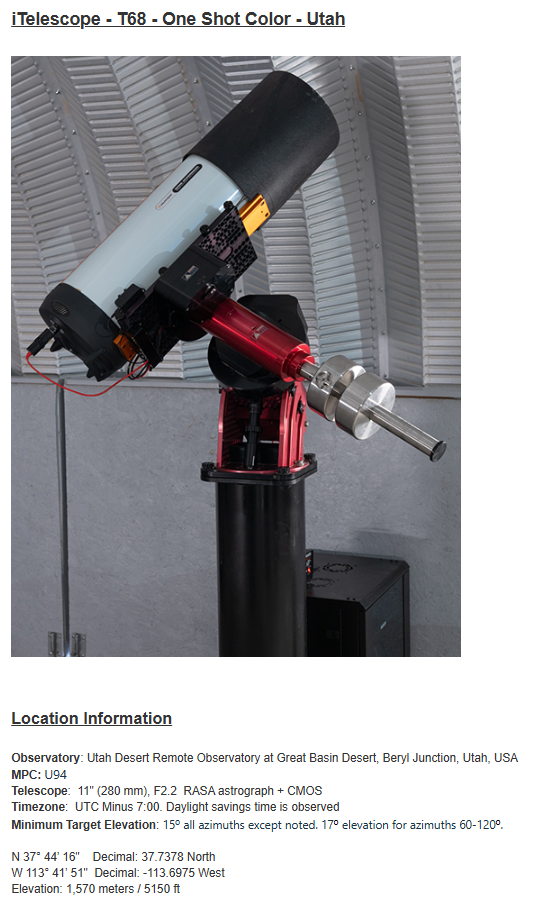
\includegraphics[width=0.6\textwidth]{Telescope1.png}
    \caption{Utah Telescope location and specifications.\cite{utahscope}}
    \label{telescope2}
\end{figure}
\newpage
When planning observations, astronomers must account for:
\begin{itemize}
    \item Astronomical sunset: The time when the sky is sufficiently dark for observations (occurring later than civil sunset).
    \item Stellar coordinates of target: The azimuth and elevation of the target object, obtainable via databases like SIMBAD.
    \item Telescope Location: Confirm the target is visible from the location of the observatory
\end{itemize}
Note that the unique identifiers assigned by the Minor Planets Center (MPC) or International Astronomical Union (IAU) for tracking observational data in multi-site studies.\cite{utahscope}
\section{Telescope Operation}
Modern telescopes function as highly specialized cameras equipped with large lenses and filters. The transition from naked-eye observations to camera-based imaging represents a significant advancement in astronomy. To capture faint celestial objects, telescopes use long exposure times, allowing the sensor to accumulate light over extended periods (often hundreds of seconds). The telescope referenced in \cite{utahscope} employs two primary imaging technologies.

\begin{figure}[H]
    \centering
    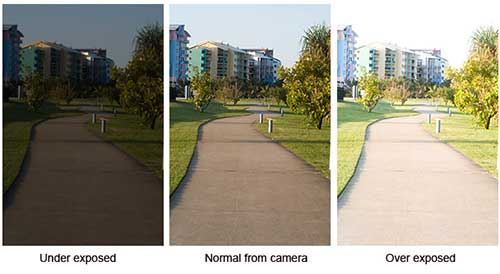
\includegraphics[width=0.6\textwidth]{Exposure1.jpg}
    \caption{Example of long-exposure imaging in astronomical observations.}
    \label{Exposure2}
\end{figure}

\section{Astrographs}
Astrographs are specialized telescopes optimized for wide-field imaging, making them ideal for:
- Stellar classification surveys,
- Tracking fast-moving objects (e.g., asteroids, comets),
- Amateur astronomy.

By deploying multiple astrographs with different filters, astronomers can quickly determine a star's peak emission wavelength and, consequently, its temperature. Most wide-field images of the night sky are captured using astrographs. These instruments often employ CMOS sensors for high-frequency imaging. Notably, the term "telescope" extends beyond optical instruments to include radio telescopes, ultraviolet telescopes, and even gravitational-wave detectors like LIGO.

\section{CMOS Sensors in Astrographs}
Complementary Metal-Oxide-Semiconductor (CMOS) sensors are the backbone of modern astronomical imaging. Their operation relies on the photoelectric effect, first explained by Albert Einstein, which describes how photons incident on a charged surface liberate electrons with energy proportional to the photons' frequency.

\begin{figure}[H]
    \centering
    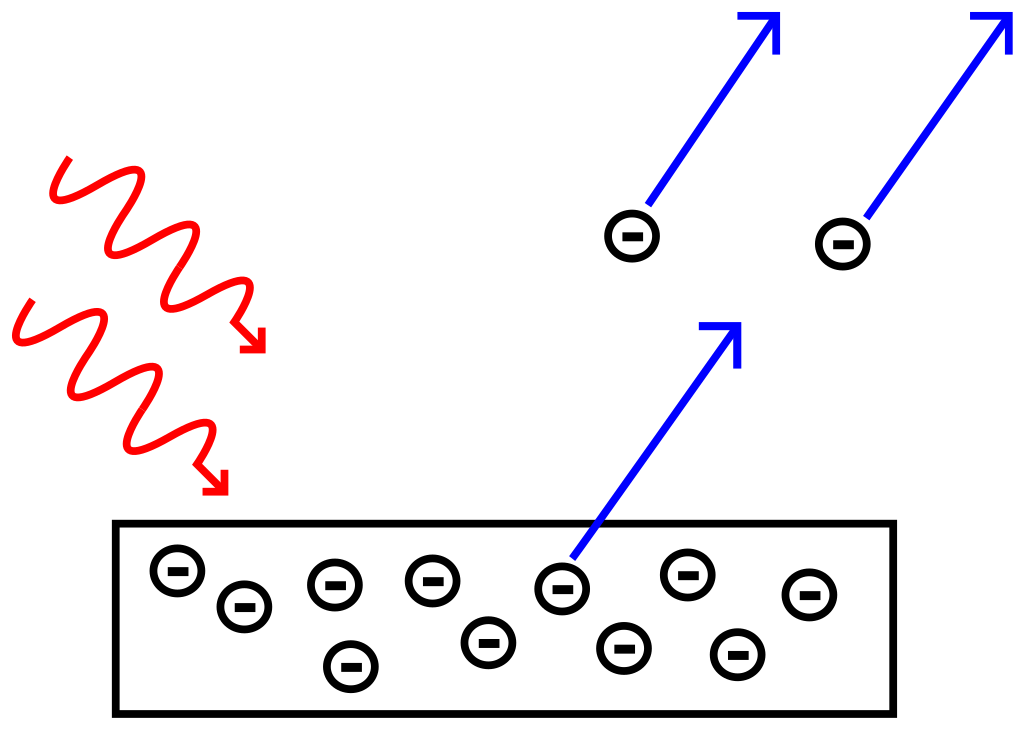
\includegraphics[width=0.6\textwidth]{Photoelectric_effect.svg.png}
    \caption{The photoelectric effect: incoming photons (red) excite electrons on a charged surface, generating a measurable current.\cite{pe1}}
    \label{pe2}
\end{figure}

The Utah telescope's specifications (Figure \ref{utah3}) include details about its CMOS sensor, such as the manufacturer and sensor design. CMOS sensors consist of microscopic lenses and color filters (typically RGB channels) fabricated as specialized integrated circuits (ICs). These components require precision manufacturing techniques due to their small scale and sensitivity.

\begin{figure}[H]
    \centering
    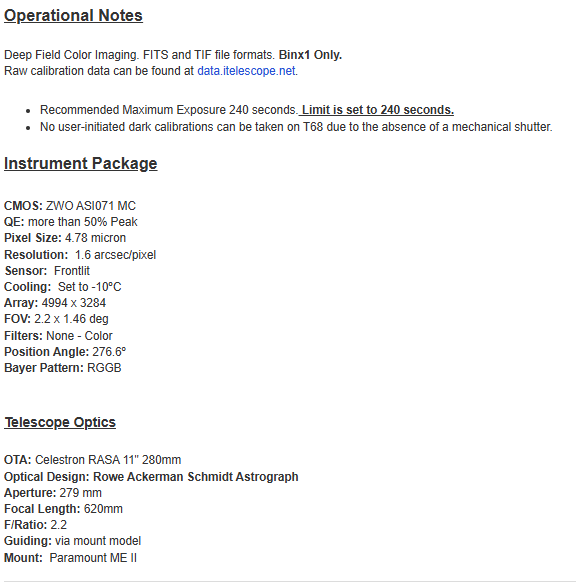
\includegraphics[width=0.6\textwidth]{Utah2.png}
    \caption{CMOS sensor and lens specifications for the Utah telescope.\cite{utahscope}}
    \label{utah3}
\end{figure}

\subsection{Quantum Efficiency (QE)}
Quantum efficiency measures a sensor's ability to convert incident photons into electrons. Manufacturers test CMOS sensors by exposing them to monochromatic light (single-wavelength) and measuring the resulting current. The QE curve in Figure \ref{qe1} shows the sensor's efficiency across different wavelengths, peaking at 50\% for 525 nm light. The four bands correspond to the sensor's color channels, with the red channel exhibiting higher sensitivity at infrared wavelengths.

\begin{figure}[H]
    \centering
    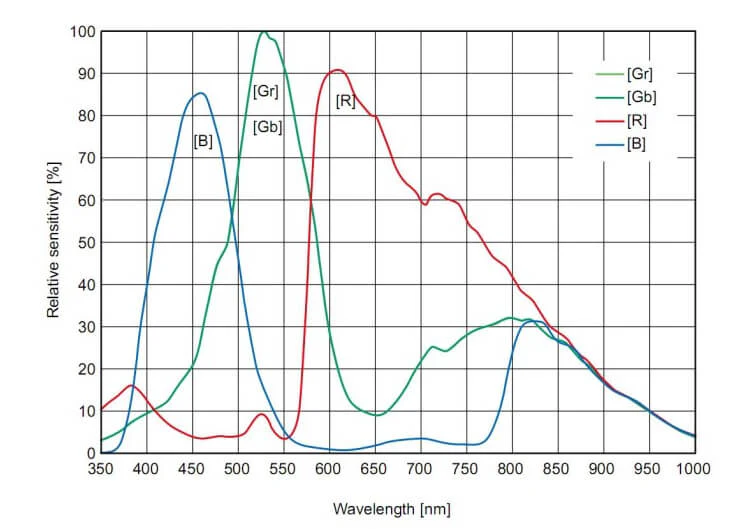
\includegraphics[width=0.6\textwidth]{QECurve.png}
    \caption{Quantum efficiency curve for the CMOS sensor in \ref{utah3}. The peak QE of 50\% occurs at 525 nm.\cite{cam1}}
    \label{qe1}
\end{figure}

\section{Instrument Package}
The telescope's imaging system comprises approximately 16 million CMOS pixels, each measuring 4.78 microns. The resolution is determined by the pixel size and the telescope's optical design. The term "arcsec/pixel" refers to the angular size of the sky imaged by each pixel, with stellar coordinates measured in degrees, arcminutes (1° = 60'), and arcseconds (1' = 60"). For the telescope in \ref{telescope2}, each pixel covers 1.6 × 1.6 arcseconds, and the full sensor array (4994 × 3284 pixels) captures a field of view (FOV) of 2.2 × 1.46 degrees.

Key specifications include:
\begin{itemize}
    \item Front-lit sensor: A design choice affecting QE (backlit sensors offer higher efficiency but are more expensive). 
    \item Cooling system: Maintains cool temperature because QE is affected by temperature.
    \item Filters: Available for specific optical bands or unfiltered observations.
    \item Bayer pattern: The RGBG pixel arrangement used in color imaging, each pixel has 4 smaller pixels arranged in a square, this is why the legend in \ref{qe1} has 4 items and 3 lines as 2 are identical.
\end{itemize}

\section{Optical Design}
Telescope optics rely on geometric principles to focus light. The Optical Tube Assembly (OTA) in Figure \ref{rasa1} illustrates a common design: light enters through a 279 mm aperture, reflects off a parabolic mirror, and converges onto a central lens or sensor. The focal length (distance from the mirror to the focal point) determines the system's light-gathering capability. The focal ratio (f/2.2 in this case) is the ratio of focal length to aperture radius. A lower focal ratio enables shorter exposures but may saturate bright objects, while higher ratios are better suited for dim targets.

\begin{figure}[H]
    \centering
    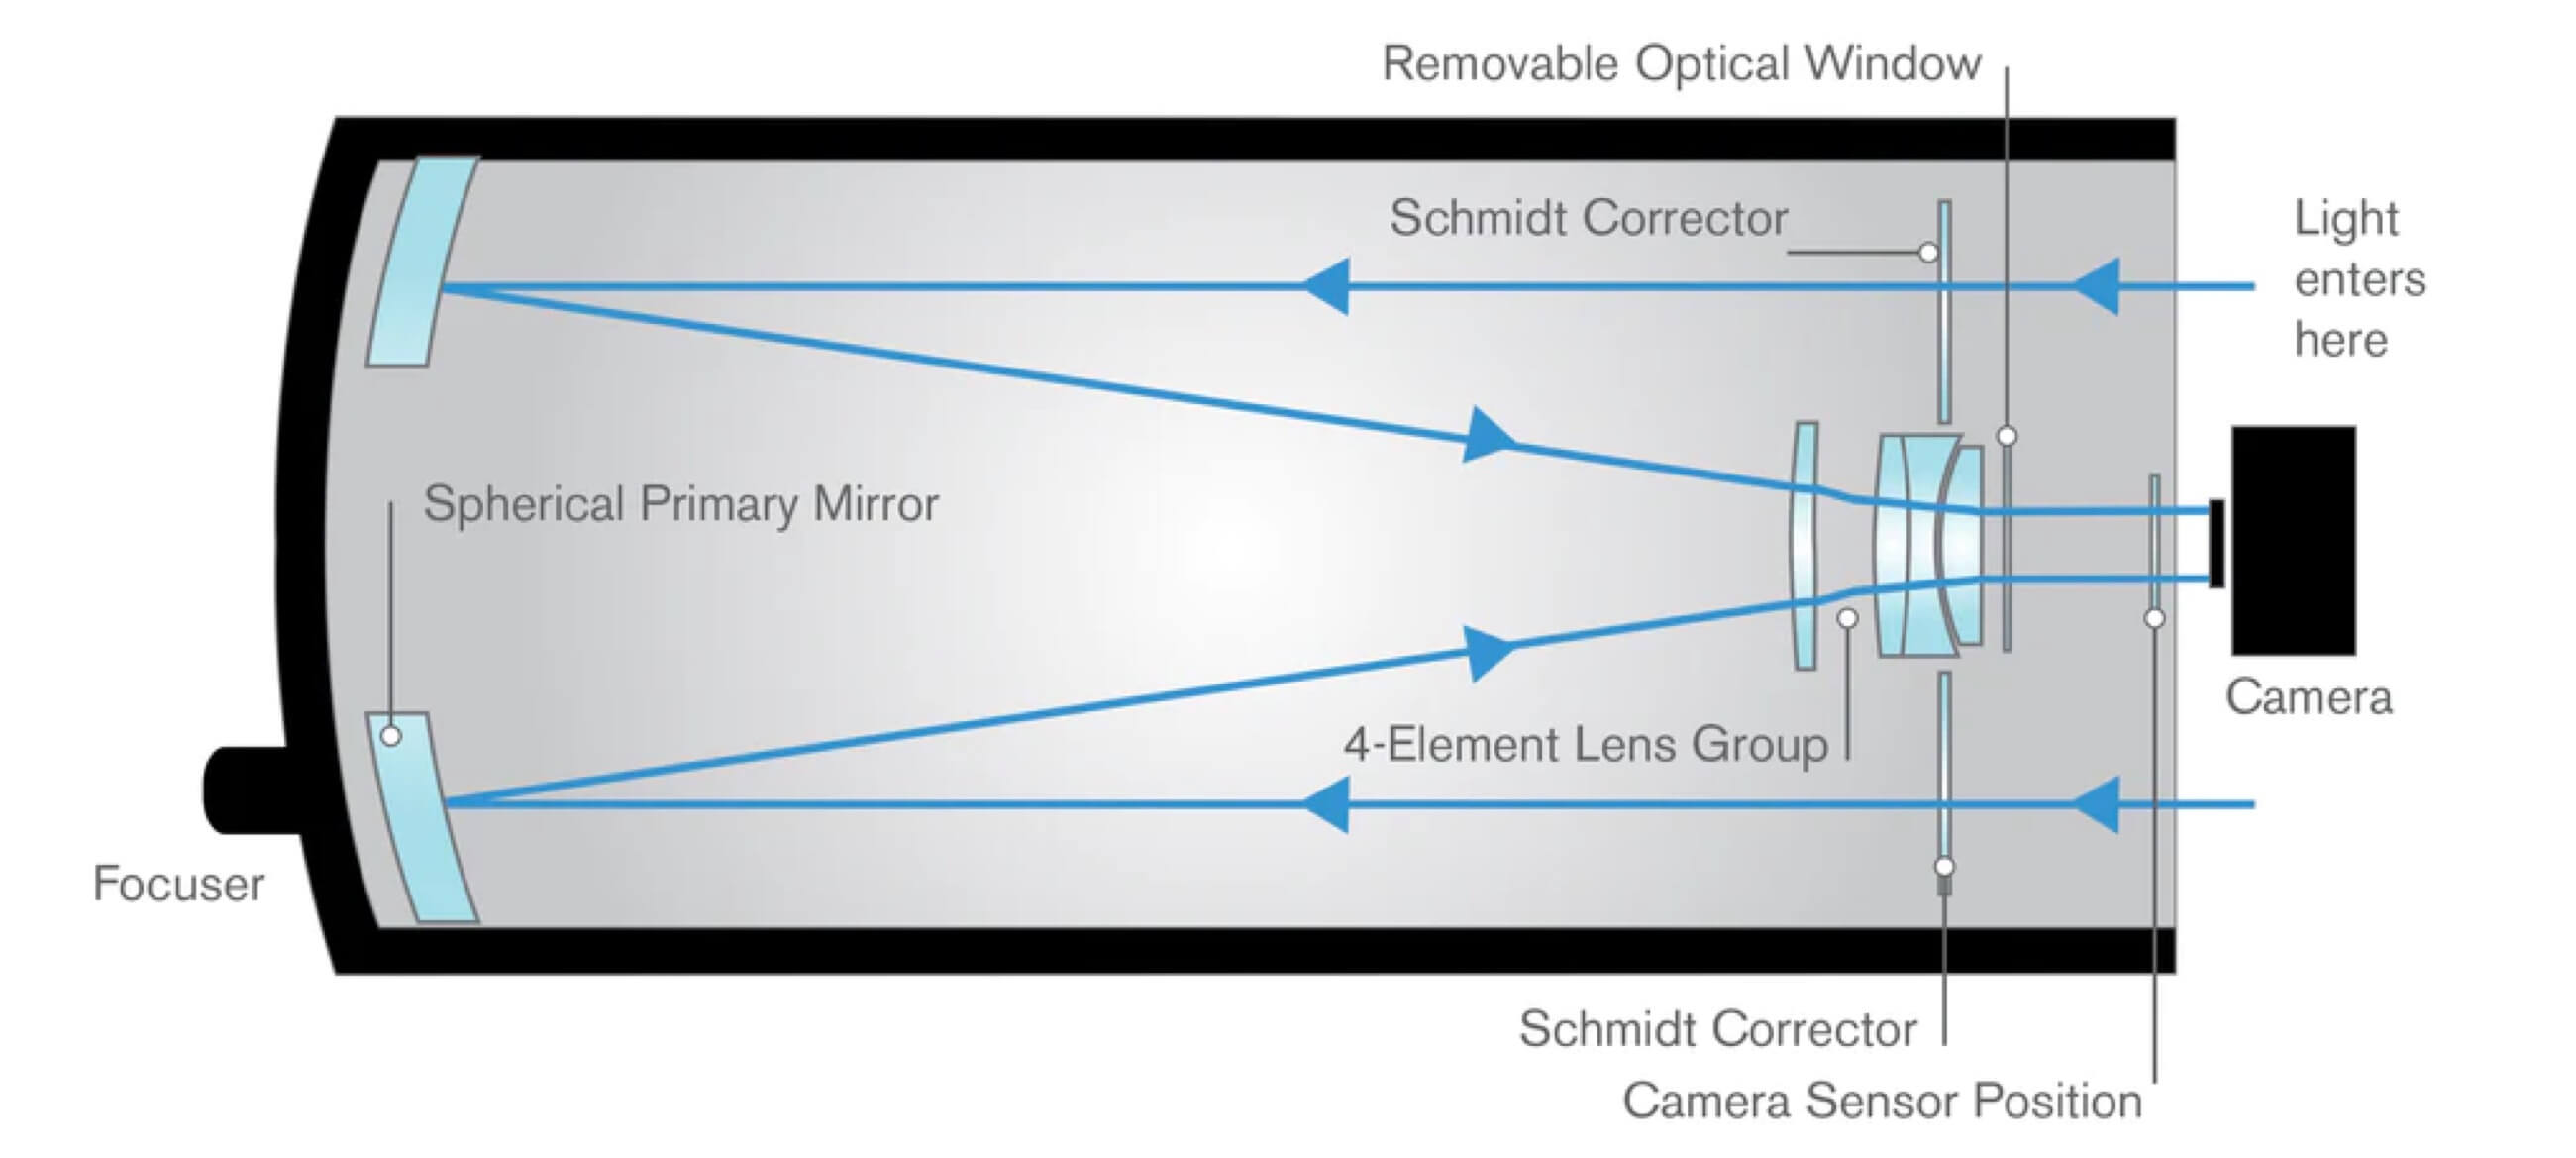
\includegraphics[width=0.6\textwidth]{RASA_Diagram.jpg}
    \caption{Optical Tube Assembly (OTA) design: light reflects off a parabolic mirror to a central sensor.\cite{rasa}}
    \label{rasa1}
\end{figure}
The mount and guiding system stabilize and position the telescope, ensuring accurate tracking of celestial objects. This article will identify differences, explaining them and explaining why astronomers may use this instead. 

\section{Photometry}
iTelescope also offers research telescopes that can do Photometry, this is the scientific measurement of light and photons coming from stars. This is a more expensive and provides more indepth measurement. Instead of a CMOS sensor or camera, this uses Charge-Coupled Device with Nighttime AntiBloom Guard(NABG), this is specialized for deep sky observation. This telescope has a much smaller FOV, less than 1 square degree(37 x 37 arcmin). The pixels are significantly smaller and thus makes the resolution much finer. This telescope also has many narrow band filters to isolated different optical bands and some special filters isolating specific light sources. This telescope is great for making measurements across many different wavelengths to determine the spectrum of emission of stars. Its important to note the F/Ratio is 9, this is much higher than \ref{utah2} and is needed to make effective deep sky measurements. This telescope will require longer exposures for each image.

\begin{figure}[H]
    \centering
    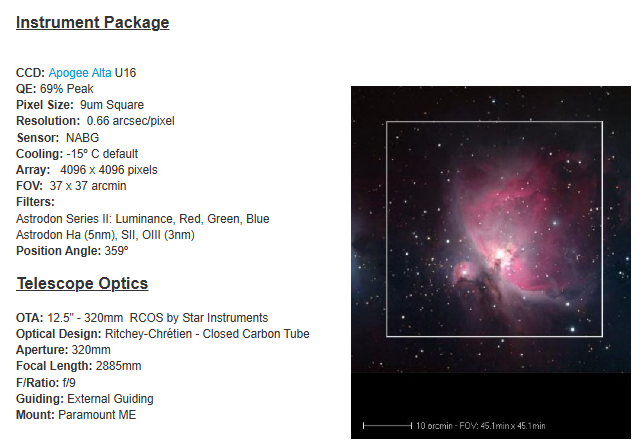
\includegraphics[width=0.6\textwidth]{Telescope2.png}
    \caption{Summary of T-33 instrument package\cite{scope2}}
    \label{photo1}
\end{figure}
\section{iTelescope Services}\cite{session_billing}
\begin{itemize}
    \item Premium telescopes: Offer advanced filters and higher-quality sensors.
    \item Subscription plans: Plan-40 and Plan-60 cater to individuals, while professional plans support research.
    \item Session billing Hourly rate for live control (recommended for experts).
    \item Exposure billing: Pay only for imaging time (e.g., three 300-second exposures = 15 minutes billed).
  
\end{itemize}
Researchers should evaluate whether they need scientific data collection or casual astrophotography. Always consider that real-time measurement is not instantaneous, to find the peak emission of a star, you will need to take multiple exposures taking 3-5 minutes and then will need data processing to extract the data. As always, there are tutorials on iTelescope for using their portal and reading the data output. It is encouraged to simply request exposures and not live control of the telescope.
\newpage
\section{References}
\bibliography{AstroTools.bib}
\bibliographystyle{ieeetr}
\end{document}